\documentclass{article}


% if you need to pass options to natbib, use, e.g.:
%     \PassOptionsToPackage{numbers, compress}{natbib}
% before loading neurips_2023


% ready for submission
\usepackage[preprint]{neurips_2023}


% to compile a preprint version, e.g., for submission to arXiv, add add the
% [preprint] option:
%     \usepackage[preprint]{neurips_2023}


% to compile a camera-ready version, add the [final] option, e.g.:
%     \usepackage[final]{neurips_2023}


% to avoid loading the natbib package, add option nonatbib:
%    \usepackage[nonatbib]{neurips_2023}


\usepackage[utf8]{inputenc} % allow utf-8 input
\usepackage[T1]{fontenc}    % use 8-bit T1 fonts
\usepackage{hyperref}       % hyperlinks
\usepackage{url}            % simple URL typesetting
\usepackage{booktabs}       % professional-quality tables
\usepackage{amsfonts}       % blackboard math symbols
\usepackage{nicefrac}       % compact symbols for 1/2, etc.
\usepackage{microtype}      % microtypography
\usepackage{xcolor}         % colors
\usepackage{amsmath,amssymb}
\usepackage{listings,graphicx}
\usepackage{algorithm}
\usepackage[noend]{algpseudocode}

\title{Report for Planning a Path for a Vacuum Cleaner Agent in a Dynamic Environment}


% The \author macro works with any number of authors. There are two commands
% used to separate the names and addresses of multiple authors: \And and \AND.
%
% Using \And between authors leaves it to LaTeX to determine where to break the
% lines. Using \AND forces a line break at that point. So, if LaTeX puts 3 of 4
% authors names on the first line, and the last on the second line, try using
% \AND instead of \And before the third author name.


\author{%
  Matthew Callahan\\
  \And
  Suphalerk Lortaraprasert
  % examples of more authors
  % \And
  % Coauthor \\
  % Affiliation \\
  % Address \\
  % \texttt{email} \\
  % \AND
  % Coauthor \\
  % Affiliation \\
  % Address \\
  % \texttt{email} \\
  % \And
  % Coauthor \\
  % Affiliation \\
  % Address \\
  % \texttt{email} \\
  % \And
  % Coauthor \\
  % Affiliation \\
  % Address \\
  % \texttt{email} \\
}


\begin{document}


\maketitle


\begin{abstract}

\end{abstract}

\section{Introduction}

In this project, the focus lies on simulating an efficient path for a vacuum cleaning robot within dynamic environments. The diversity of real-world rooms and their varying layouts renders fixed paths impractical for universal application. Thus, our aim is to develop a solution that adapts to changing environments, ensuring optimal cleaning efficiency regardless of room type or layout. This simulation endeavors to explore and implement strategies that enable the robot to navigate dynamically and effectively, enhancing its utility in real-world scenarios.

We note that even on a $3\times 3$ board, there are at least $2^9$ possible belief states. This means that producing a complete plan is not feasible for reasonable problems in reasonable time. 
\section{Agent Descriptions}
The available actions of the agent are to clean the square it is on, to move forward one square, to turn left (counter clockwise) $90^\circ$, to turn right (clockwise) $90^\circ$, and to turn off. Since there is no cost for making actions, no agent that we designed was instructed to turn off.

The agents have the ability to detect whether the square they are on are clean or dirty with 100\% reliability. Additionally, they can detect if they are facing a wall and if they are on the square they started on. This last sensor input was not determined to be useful for our purposes. 
\subsection{Memoryless deterministic reflex agent}
This agent was designed to have only deterministic rules for actions based solely on the current precepts. When designing this, we determined that the highest priority action was to clean the square it was on if it found the square to be dirty. Otherwise, it would turn if it found itself facing a wall, and advance otherwise. The design is shown explicitly in Algorithm~\ref{alg:SimpleAgent}. Since it cannot record previous precepts, it does not have a way to translate over a column and therefore the best it can do is to clean the edges of the space it is in.

Under the constraints provided, this is the optimal agent that can be constructed regardless of the environment it is in. Therefore if the room had obstacles placed in it the same agent would be used. 
\begin{algorithm}[h]
  
  \caption{Programmatic Description of Simple Reflex Agent}
  \begin{algorithmic}[1]
    
    \For {timestep $t$ until termination}
    \If {on dirty tile}
    \State clean tile 
    \EndIf
    \If{ not on dirty tile and facing wall}
    \State turn clockwise
    \EndIf
    \If{not facing wall and not on dirty tile}
    \State move forward
    \EndIf
    \EndFor
  \end{algorithmic}
  \label{alg:SimpleAgent}
\end{algorithm}
\subsection{Memoryless random reflex agent}
The random reflex agent was designed to allow the vacuum to rotate even if there is no wall in front of it. Random systems work on a probabilistic basis. This allows the vacuum to choose between turning left and right with equal chance when facing a wall or even in the case where there are no obstructions. In general, This random agent prioritizes forward movement to increase performance, it weights moving forward compared to turning with a ratio of 85:15.
The formulation is made explicit in Algorithm \ref{alg:RandomAgent}. One advantage of random agents is that they can have a best-case performance comparable to an agent with much higher memory to define a model. In addition, it is much easier to design such an agent and the same agent can work in many different environments, even with obstacles. The dissadvantage is that lower bounds on performance are hard to make and expected performance is often lower than a well designed agent. 


\begin{algorithm}[h]
  
  \caption{Programatic Description of Simple Reflex Agent}
  \begin{algorithmic}[1]
    
    \For {timestep $t$ until termination}
    \If {on dirty tile}
    \State clean tile 
    \EndIf
    \State random = (random action of agent) //move forward with 85 possibility and turning with 15 possibility
    \If {random equal move forward} 
      \If{not facing wall and not on dirty tile}
      \State move forward
      \Else 
      \State turn clockwise or counterclockwise //random with 50:50
      \EndIf
    \Else { random equal move forward}  
      \If{ not on dirty tile and facing wall}
      \State turn clockwise or counterclockwise //random with 50:50
      \EndIf
      \EndIf
     
    \EndFor
  \end{algorithmic}
  \label{alg:RandomAgent}
\end{algorithm}


\subsection{Low-memory deterministic reflex agent}
The low-memory deterministic reflex agent was designed such that it would clean the room column by column, making a u-turn in alternating directions when it reaches a wall. With the way it was designed it needs three bits of memory to function. It performs very well in the empty room scenario, but when internal walls are introduced it does not perform as well because the aditional walls cause problems with the parity of alternating turns and since it is designed to clean via columns it has difficulty entering rooms with doors on the sides or on the top. The agent is explained in detail in Algorithm ~\ref{alg:ThreeBit}

With more memory the agent could remember all the spaces it had yet to travel to and could plan a path towards these regions. This would allow perfect cleaning regardless of the obstacles present.
\begin{algorithm}
  \begin{algorithmic}[1]
    \For {timestep $t$ until termination}
      \If{ on dirty tile}
        \State clean tile
      \Else 
        \If {turnState==FinishTurn}
          \State clear turnState
          \If{LeftUTurn}
            \State turn left
            \State LeftUTurn $\gets$ False
            
          \Else
            \State turn right
            \State LeftUTurn $\gets$ True
          \EndIf
        \EndIf
        \If{Detect Wall}
          \State turnState $\gets$ ShiftOver
          \If {LeftUTurn}
            \State turn left
          \Else
            \State turn right
          \EndIf
          
        \Else
          \If {turnState == ShiftOver}
            \State turnState $\gets$ FinishTurn
            \State move forward
          \Else
            \State move forward
          \EndIf
        \EndIf
      \EndIf
    \EndFor
  \end{algorithmic}\caption{The structure of the low memory agent as if-then rules}
  \label{alg:ThreeBit}
\end{algorithm}

\subsection{New agent that can look next cell denpend on input }
new wwwwwwwwwwwwwwwwwwwwwwwwwwwwwwww

\section{Environment setup}

In our experimental setup, we categorize environments into three types: NOWALL, FIXWALL, and RANDOMWALL.

\subsection{NOWALL Environment:} This type of environment is characterized by open spaces without any fixed obstacles or walls. It represents scenarios where the robotic vacuum cleaner has unrestricted movement and can navigate freely across the entire area.

\subsection{FIXWALL Environment:} In contrast to NOWALL environments, FIXWALL environments include fixed obstacles or walls that create defined pathways and rooms within the space. This setup simulates typical indoor environments where rooms are separated by walls and furniture, influencing the robot's path planning and navigation strategy.

\subsection{RANDOMWALL Environment:} This environment type introduces variability by including randomly placed obstacles or walls within the space. The placement of these obstacles varies across different runs or simulations, mimicking dynamic and unpredictable real-world environments. This setup challenges the robot's ability to adapt its cleaning route dynamically in response to changing environmental conditions.


Each environment type serves a specific purpose in our experiments: NOWALL for testing unrestricted navigation scenarios, FIXWALL for evaluating path planning efficiency in structured environments, and RANDOMWALL for assessing adaptability and robustness in unpredictable settings. By systematically testing our robotic vacuum cleaner in these varied environments, we aim to develop and refine intelligent algorithms that optimize cleaning routes and enhance overall performance across diverse real-world conditions.

\section{Experimental setup}
The agent starts at the bottom left hand corner of a 10 by 10 grid facing up. It can advance one square in the direction it is facing, and can turn $90^\circ$ either direction during a time step. The agent was run for 500 time steps with the number of clean tiles recorded at each step. The random agent was run 50 times with the room and agent reset after 500 time steps each time.

There were two configurations of room. One configuration consisted of 10 by 10 cells connected at the edges  all initially marked as dirty. The second consisted of four rooms with doors near the center of the room. 

% please include more detail about the room with extra walls

The room with internal walls has walls in the middle such that one room is of size 5 and the other is of size 4. There are four gaps in these internal walls right around the intersection between the walls.  The simulation was run for 500 time steps and repeated 50 times for the random agent. 




\section{Results}
Here we include several figures of number of clean cells vs. number of time steps.  In our experiments, the random agent took 500 steps to clean 90\% of the area of it succeeded in doing so at all. it failed to clean 90\% more than five times, so the average is also 500. This is explained in table~\ref{tab:randomPerf}


\begin{table}
  \caption{Sample table title}
  \label{tab:randomPerf}
  \centering
  \begin{tabular}{lll}
    \toprule
    Setting     & Top 45 Average     & Mode \\
    \midrule
    Empty room &  500 & 500    \\
    Internal walls     & 500 & 500     \\
    \bottomrule
  \end{tabular}
\end{table}

\begin{figure}[h!]
  \centering

  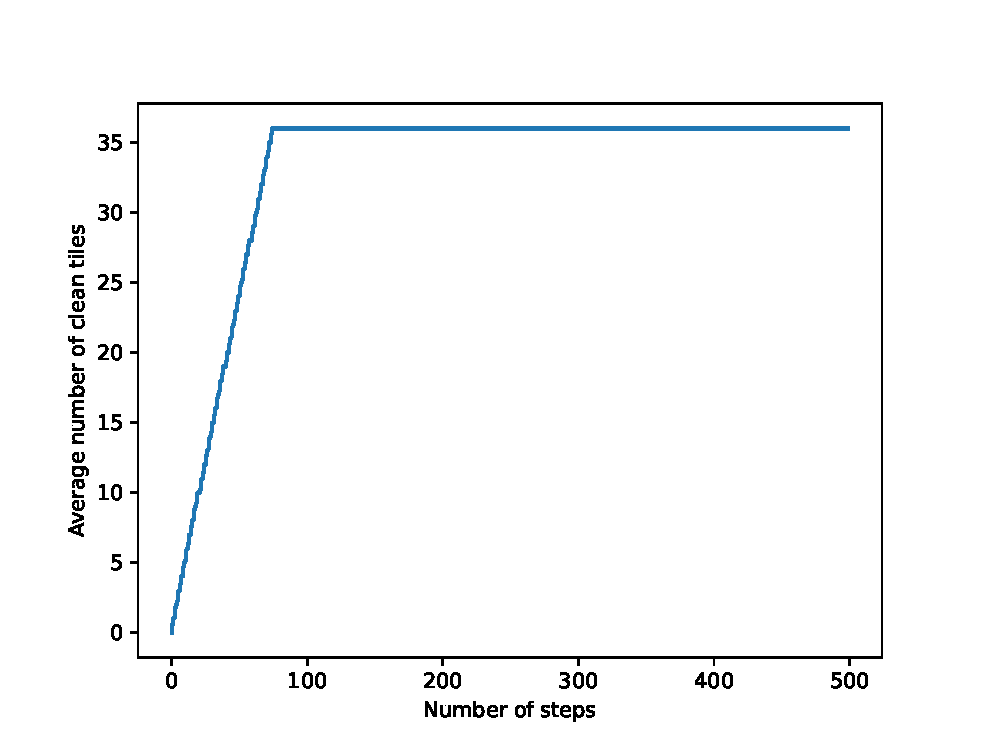
\includegraphics[width=0.8\textwidth]{SimpleNoWallPerformance}
  \caption{Performance of simple agent in empty room. The agent is unable to clean 90\% of the area isnce it is unable to leave the perimeter of the room. }
  \label{fig:SimpleNoWall}
\end{figure}

\begin{figure}[h!]
  \centering
  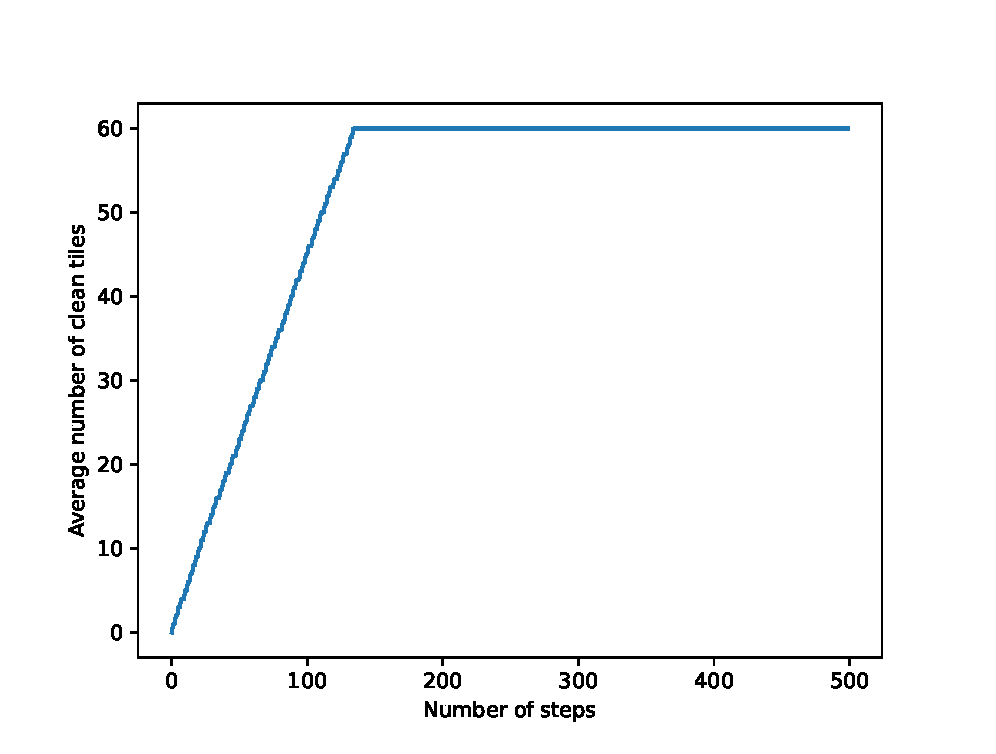
\includegraphics[width=0.8\textwidth]{SimpleExtraWallPerformance}
  \caption{Performance of simple agent in room with internal walls. The additional walls provide aditional places for the agent to turn, increasing its performance. }
  \label{fig:SimpleExtraWall}
\end{figure}
\begin{figure}[h!]
  \centering
  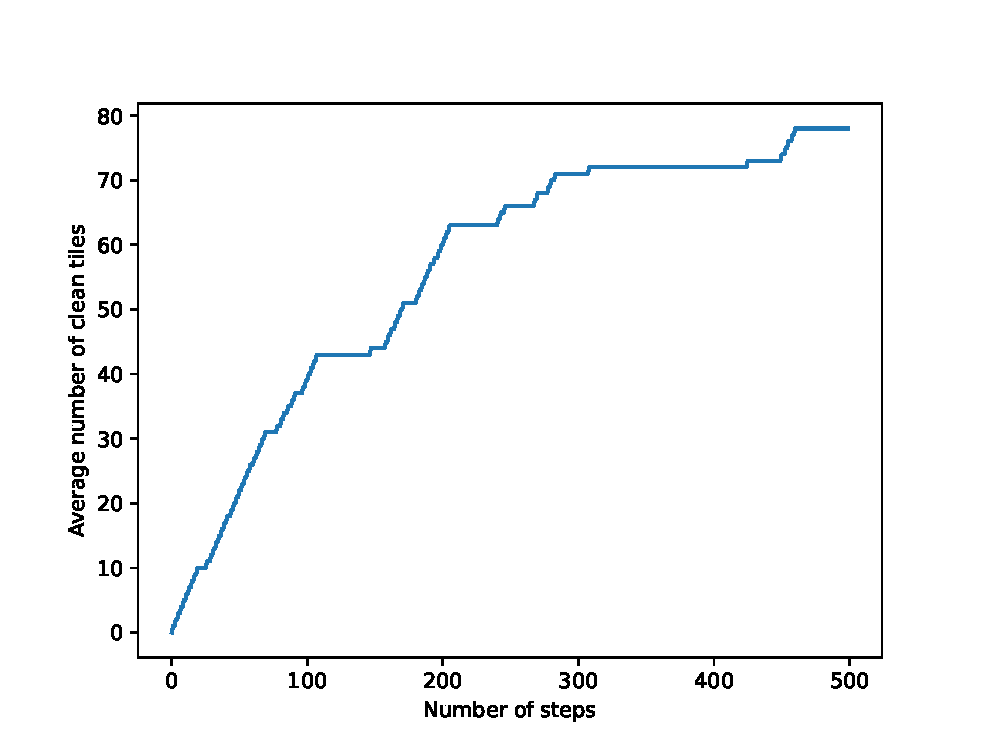
\includegraphics[width=0.8\textwidth]{RandomNoWallPerformance}
  \caption{Performance of random agent on room without internal walls. This does not clean the entire region in the 500 cycles.  }
  \label{fig:1}
\end{figure}
\begin{figure}[h!]
  \centering
  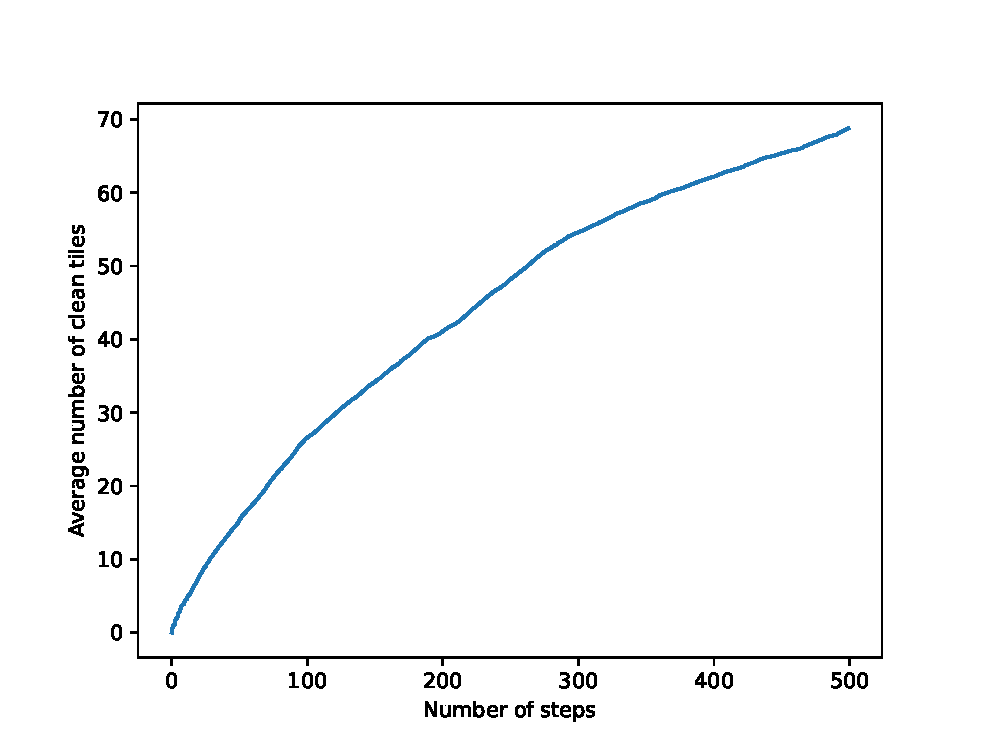
\includegraphics[width=0.8\textwidth]{RandomExtraWallPerformance}
  \caption{Performance of random agent with internal walls. This performs roughly as well as without the internal walls but the number of clean tiles is smaller since there are fewer tiles (some are displaced by walls).  }
  
\end{figure}



\begin{figure}[h!]
  \centering
  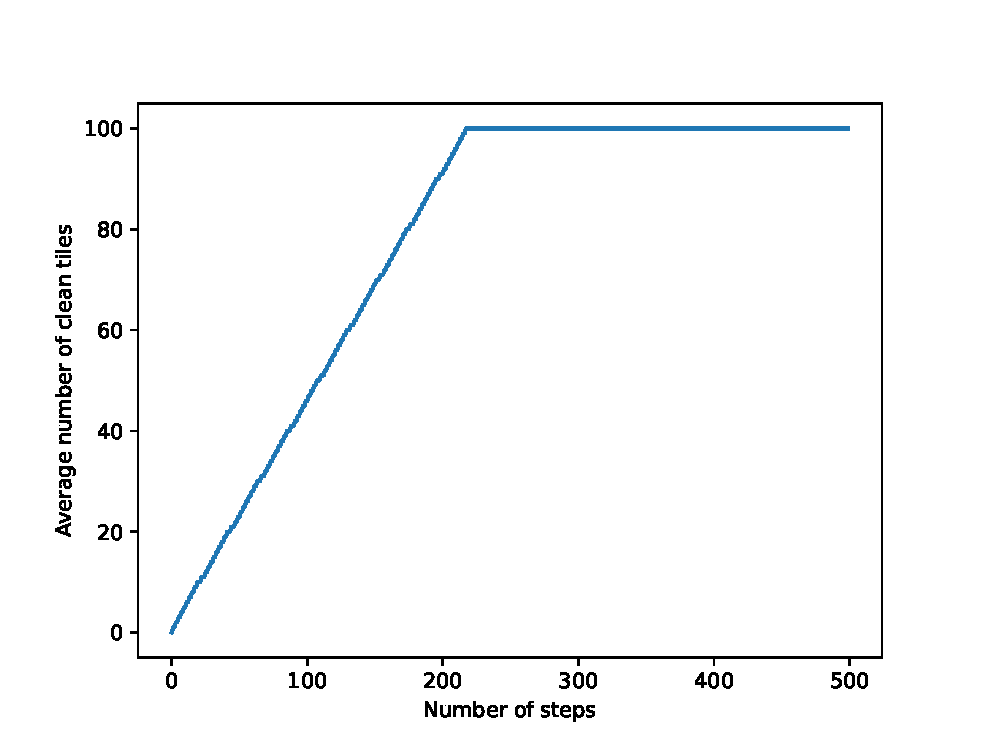
\includegraphics[width=0.8\textwidth]{FancyNoWallPerformance}
  \caption{Three bit agent performance in the empty room. The agent quickly cleans every tile. }
\end{figure}

\begin{figure}[h!]
  \centering
  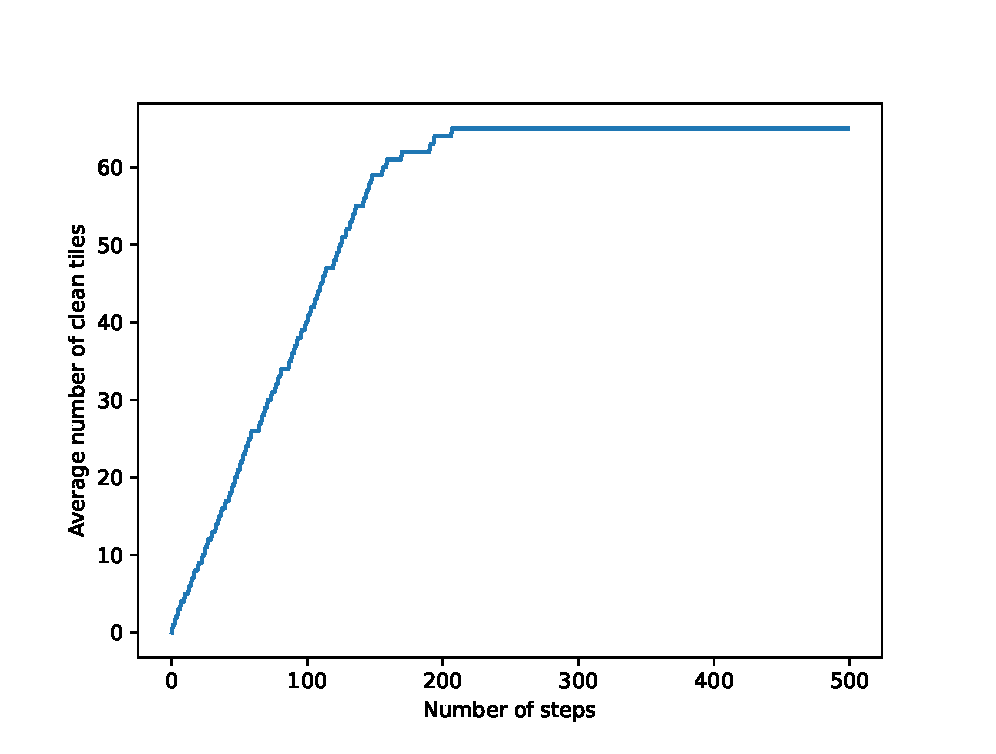
\includegraphics[width=0.8\textwidth]{FancyExtraWallPerformance}
  \caption{Three bit agent performance in room with additional walls. The agent gets turned away from the bottom right room and thus fails to clean a quarter of the room. }
  \label{fig:FancyExtraWall}
\end{figure}
\section{Discussion}
% Answer the remaining questions not answered in earlier sections

We were surprised by how difficult the low-memory agent was to implement successfully and that it performed so poorly when additional walls were introduced.


\subsection It should compare at least two different approaches and try to conclude some hypothesis: say a method X works better than Y under these conditions. 



\end{document}